
\documentclass[10pt]{article}

% Use reasonably small margins
\usepackage{fullpage}

% for various math utilities
\usepackage{amsmath}
\usepackage{amssymb}
\usepackage{commath}
\usepackage{cancel}
\usepackage{breqn}
\usepackage{comment}
\usepackage{esvect}
\usepackage[T1]{fontenc}

% provides non-italicised Greek letters in text
\usepackage[euler]{textgreek}

% provides the \includegraphics command
\usepackage{graphicx}

% allows figure environments to be placed in exact locations
\usepackage{float}

% Bold caption labels, and give captions increased margins
\usepackage[labelfont=bf, margin=1cm]{caption}
\usepackage{subcaption}

% allows for configurable source code listings
\usepackage{listings}
\usepackage{color}
\definecolor{dkgreen}{rgb}{0,0.6,0}
\definecolor{gray}{rgb}{0.5,0.5,0.5}
\definecolor{red}{rgb}{0.8,0,0}
\lstset{frame=tb,
  language=C,
  aboveskip=3mm,
  belowskip=3mm,
  showstringspaces=false,
  columns=flexible,
  basicstyle={\small\ttfamily},
  numbers=left,                    % where to put the line-numbers; possible values are (none, left, right)
  numbersep=5pt,                   % how far the line-numbers are from the code
  numberstyle=\tiny\color{gray},   % the style that is used for the line-numbers
  stepnumber=1,                    % the step between two line-numbers. If it's 1, each line will be numbered
  keywordstyle=\color{blue},
  commentstyle=\color{dkgreen},
  stringstyle=\color{red},
  breaklines=true,
  breakatwhitespace=true,
  breakindent=50pt,
  tabsize=4
}

\usepackage{listings}
\usepackage{color} %red, green, blue, yellow, cyan, magenta, black, white
\definecolor{mygreen}{RGB}{28,172,0} % color values Red, Green, Blue
\definecolor{mylilas}{RGB}{170,55,241}
\renewcommand{\ttdefault}{pcr} % selects Courier font
% allows hyperlinks
\usepackage{hyperref}

\DeclareMathOperator*{\argmin}{arg\,min\:}


\begin{document}

\begin{center}
\textsc{\huge \bfseries Computer Lab 3} \\[1cm]
\textsc{\huge \bfseries EM Algorithm for a Simple Shape Model} \\[2cm]
\textsc{\large \bfseries Morhunenko Mykola}\\[13cm]

\textup{\large \bfseries FACULTY OF ELECTRICAL ENGINEERING,\\ CZECH TECHNICAL UNIVERSITY IN PRAGUE}
\end{center}
\newpage



*The notation used is the same as in the assignment document.

\section{Assignment 1}
\label{sec:ass1}
\begin{figure}[H]
  \begin{center}
      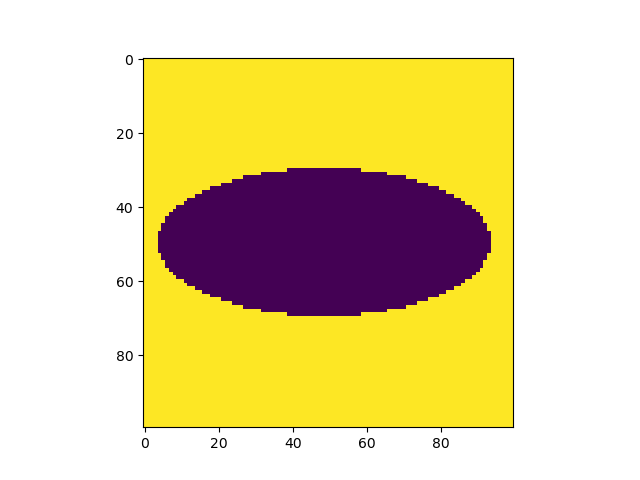
\includegraphics[width=0.5\textwidth]{fig/elipsa.png}
  \end{center}
      \caption{The shape model learned by the EM algorithm, assignment 1.}
      \label{fig:sun}
\end{figure}

Let us first consider the following simpler task: the ML estimate
of the shape s and the 2-tuple ($\eta_0$, $\eta_1$) in case all images where generated from the
same shape pose. The task reads
\begin{equation}
    \frac{1}{m} \sum_{x \in \mathcal{T}^m}{ \log p(x;s, \eta)} \rightarrow{} \max_{s, \eta}.
\end{equation}
Substituting the model:
\begin{equation}
    \begin{aligned}
        \frac{1}{m} \sum_{x \in \mathcal{T}^m} { \log p(x;s, \eta)} = \\ 
        \frac{1}{m} \sum_{x \in \mathcal{T}^m} { \langle x, \eta(s) \rangle - n_0(s)\log(1 + e^{\eta_0}) - n_1(s) \log(1 + e^{\eta_1})} = \\
        \langle \frac{1}{m} \sum_{x \in \mathcal{T}} x, \eta(s) \rangle - n_0(s)\log(1 + e^{\eta_0}) - n_1(s) \log(1 + e^{\eta_1}) = \\
        \langle \psi, \eta(s) \rangle - n_0(s)\log(1 + e^{\eta_0}) - n_1(s) \log(1 + e^{\eta_1})
     \end{aligned}
\end{equation}
where $\psi = \frac{1}{m} \sum_{x \in \mathcal{T}^m} x$, so all you need from the data is the average image.

As far as this can not be solved by gradient ascent because the shape parameter is discrete,
the algorithm for optimisation is, as was discussed in seminars - something that can be called batch gradient ascent.
Firstly optimise with respect to $\eta$ in a closed form, then with respect to $s$ also in a closed form.
The optimisation with respect to $\eta$ is straightforward - take the derivative, make it equal to 0 and express $\eta$'s:
\begin{equation}
    \eta_i = \log \frac{ \sum_{x \in \mathcal{T}} {x_{\eta_i}}}{n_i(s) - \sum_{x \in \mathcal{T}} x_{\eta_i}}.
\end{equation}
It can not be solved as this for the shape because the shape is a binary image, so it was also done straightforward:
\begin{equation}
    \begin{aligned}
        s_0 =  \langle x, \eta_0(s) \rangle - n_0(s)\log(1 + e^{\eta_0}) \\
        s_1 =  \langle x, \eta_1(s) \rangle - n_1(s)\log(1 + e^{\eta_1}) \\
        s = s_1 > s_2,
    \end{aligned}
\end{equation}
where $s$ is a new shape, and $s_1 > s_2$ means that $s_{ij} = 1$ where $s_{1, ij} > s_{2, ij}$ and $s_{ij} = 0$ vice versa.

For the first dataset (ellipse), etas received after applying the algorithm are $(-0.405694, 0.406514)$, and the shape is in the \autoref{fig:elipsa}

\section{Assignment 2}
\label{sec:ass2}

\begin{figure}[H]
  \begin{center}
      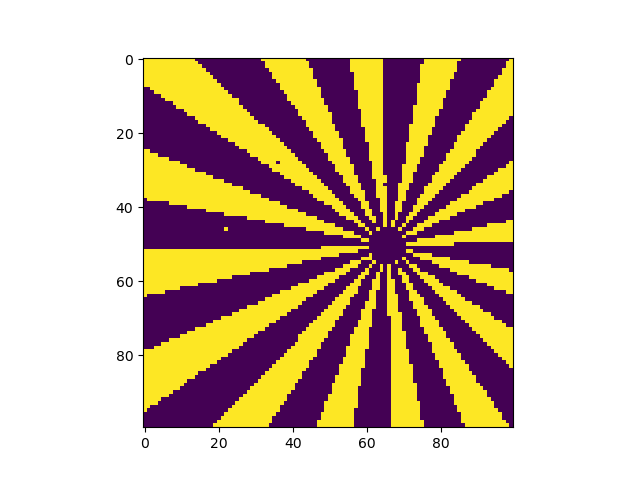
\includegraphics[width=0.5\textwidth]{fig/sun.png}
  \end{center}
      \caption{The shape model learned by the EM algorithm, assignment 2.}
      \label{fig:elipsa}
\end{figure}

\subsection{E-step}
Given the current model parameter estimates for $s, \eta$ and $\pi$, you need to compute
\begin{equation}
    a_x(r) = p(r | x; s, \eta)
\end{equation}
for each image in $x \in \mathcal{T}^m$.
These posterior probabilities can be computed by
\begin{equation}
    a_x(r) = \text{softmax}_{r}(\langle x, \eta(T_rs) \rangle + \log(\pi_r))
\end{equation}
because
\begin{equation}
    \begin{aligned}
        p(r | x; s, \eta) = \\
        \frac{p(x | r; s, \eta) p(r; s, \eta)}{p(x; s, \eta)} = \\
        \frac{\exp{[\langle x, \eta(T_rs) \rangle - n_0(s)\log(1 + e^{\eta_0}) - n_1(s)\log(1 + e^{\eta_1}) + \log{\pi_r}]}}{\sum_r{\exp{[\langle x, \eta(T_rs) \rangle - n_0(s)\log(1 + e^{\eta_0}) - n_1(s)\log(1 + e^{\eta_1}) + \log{\pi_r}]}}} = \\
        \text{softmax}_{r}(\langle x, \eta(T_rs) \rangle + \log(\pi_r))
    \end{aligned}
\end{equation}

\subsection{M-step}
Fixing the alphas from the E-step, the task needs to be solved is
 \begin{equation}
    \begin{aligned}
        \frac{1}{m}\sum_{x \in \mathcal{T}^m} \sum_r a_x(r) (\log p(x|r;s, \eta) + \log \pi_r ) \rightarrow{} \max_{s, \eta, \pi}
    \end{aligned}
 \end{equation}
 \begin{equation}
    \begin{aligned}
        \frac{1}{m}\sum_{x \in \mathcal{T}^m} \sum_r a_x(r) (\log p(x|r;s, \eta) + \log \pi_r ) = \\
        \frac{1}{m}\sum_{x \in \mathcal{T}^m} \sum_r a_x(r) (\langle x, \eta(T_rs) \rangle - n_0(s)\log(1 + e^\eta_0) - n_1(s) \log(1 + e^\eta_1)) + \log \pi_r ) = \\
        \frac{1}{m}\sum_{x \in \mathcal{T}^m} \sum_r a_x(r) (\langle x, \eta(T_rs) \rangle) - a_x(r)n_0(s)\log(1 + e^\eta_0) - a_x(r)n_1(s) \log(1 + e^\eta_1)) + a_x(r)\log \pi_r = \\
        \langle \frac{1}{m}\sum_{x \in \mathcal{T}^m} \sum_r a_x(r) T^T_r x, \eta s \rangle - \frac{1}{m}\sum_{x \in \mathcal{T}^m} \sum_r a_x(r)n_0(s)\log(1 + e^\eta_0) - a_x(r)n_1(s) \log(1 + e^\eta_1)) + a_x(r)\log \pi_r = \\
        \langle \psi, \eta s \rangle - \frac{1}{m}\sum_{x \in \mathcal{T}^m} \sum_r a_x(r)(n_0(s)\log(1 + e^\eta_0) - n_1(s) \log(1 + e^\eta_1) + \log \pi_r) = \\
        \langle \psi, \eta s \rangle - n_0(s)\log(1 + e^\eta_0) - n_1(s) \log(1 + e^\eta_1) + \frac{1}{m}\sum_{x \in \mathcal{T}^m} \sum_r a_x(r)(\log \pi_r)
    \end{aligned}
\end{equation}
where $ \psi = \frac{1}{m}\sum_{x \in \mathcal{T}^m} \sum_r a_x(r) T^T_rx $. So all needed from the data is the array $\psi$, and the maximiser for the probabilities $\pi_r$ can be found in a closed form. For $\eta$'s and $s$, the same maximiser as in \autoref{sec:ass1} can be used.

The assignment's initial parameters are chosen as written: the 2-tuple $\eta$ as in \autoref{sec:ass1}, the initial pose probabilities - uniform, the initial shape - random binary image of the same shape as images in the given dataset.
The stopping criterion for the algorithm: stop if the new shape is the same as the shape in the previous step.
, it is a good stopping criterion with only one extra execution but shows that the program will not improve anything anymore.

The final shape estimate is shown in the \autoref{fig:sun}, prior pose probabilities are $[0.2 0.3 0.3 0.2]$ and the $\eta = (-0.201618, 0.199386)$

\end{document}